\subsection{Симулация на крайни автомати чрез обобщени мрежи}

\hspace*{2.5em}В тази глава се показва как краен автомат може да бъде описан и симулиран с помощта на ОМ. Стъпка по стъпка ще се изгради връзката между състоянията и преходите на автомата и съответните елементи на ОМ, така че да е ясно как моделът се превръща в работеща схема. Разгледан е и конкретен пример на краен автомат, за който се изгражда съответната ОМ и се реална симулация с \textit{OnlineGN}. 
При разработването и анализа ще бъде следван подходът, предложен в \cite{DimitrievAutomata}.
В \cite{Atanassov1985GNFA} вече е разгледан начин за представяне на автомати чрез ОМ, но основният акцент е поставен върху теоретичното доказателство за съществуването на такова представяне. Липсва обаче конструкция, която да е директно приложима за симулация в софтуерни среди за ОМ, където биха били нужни конкретни структурни ограничения и оптимизации.

\subsubsection{Основни понятия за крайни автомати}

\paragraph*{Крайни азбуки и езици.}
\mbox{}\\
\emph{Крайна азбука} е крайно множество от символи, обикновено означаван със $\Sigma$. \emph{Низ} (или \emph{дума}) над $\Sigma$ е крайна последователност от символи от $\Sigma$. Празният низ (който не съдържа символи) се обозначава с $\varepsilon$. \emph{Език} $L$ над $\Sigma$ е произволно множество от низове над $\Sigma$, т.е. $L \subseteq \Sigma^*$ (като $\Sigma^*$ е множеството от всички низове със символи от $\Sigma$).
\paragraph*{Детерминиран краен автомат (ДКА).}
\mbox{}\\
\label{def:DFA}
\emph{Детерминираният краен автомат} (ДКА) е петорка \cite{HopcroftMotwaniUllman,Kozen}
\[
\mathcal{A} = (Q,\, \Sigma,\, \delta,\, q_{\textit{start}},\, F),
\]
където:
\begin{itemize}
  \item $Q$ е крайно множество от \emph{състояния};
  \item $\Sigma$ е крайна \emph{азбука};
  \item $\delta : Q \times \Sigma \to Q$ е \emph{функцията на прехода}, която е тотална (т.е.\ дефинирана за всяка двойка $(q,a)$ с $q \in Q$ и $a \in \Sigma$);
  \item $q_{\textit{start}} \in Q$ е \emph{началното състояние};
  \item $F \subseteq Q$ е множеството от \emph{приемащи} (или \emph{крайни}) състояния.
\end{itemize}

На \textbf{Фигура~\ref{fig:dfa_figure}} е илюстриран пример за детерминиран краен автомат.
\begin{figure}[H]
\centering
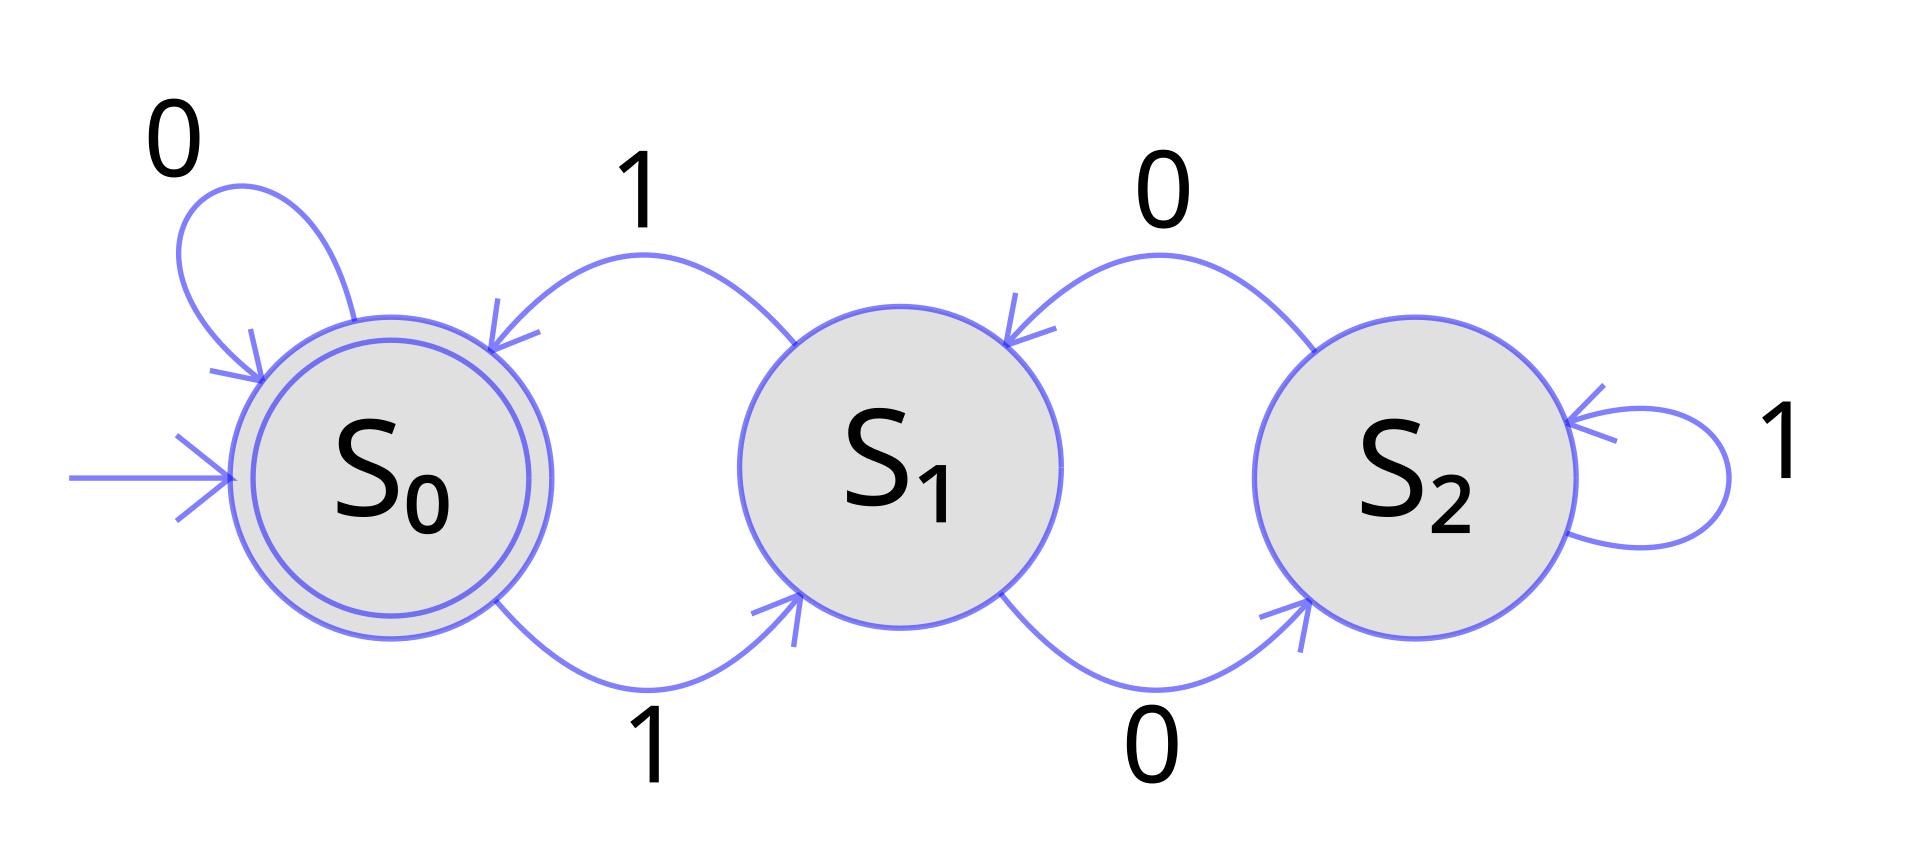
\includegraphics[width=0.6\textwidth]{4. applications/finateStateAutomationsGenNets/images/DFA.png}
\caption{Пример за детерминиран краен автомат.}
\label{fig:dfa_figure}
\end{figure}

\paragraph{Кога ДКА приема дума?}
\mbox{}\\
Нека $\alpha = a_0 a_1 \cdots a_{n-1}$ е дума над азбуката $\Sigma$. ДКА $\mathcal{A}$ \emph{приема} (или \emph{разпознава}) $\alpha$, ако съществува последователност от състояния 
\(
q_0, q_1, \dots, q_n \in Q,
\)
такава че:

\begin{itemize}
	\item началното състояние е $q_0 = q_{\textit{start}}$,
	\item за всяко $0 \le i < n$ преходът е $\delta(q_i, a_i) = q_{i+1}$,
	\item крайното състояние е $q_n \in F$.
\end{itemize}

Еквивалентно, можем да използваме разширената преходна функция \\
\(
\delta^* : Q \times \Sigma^* \to Q
\), която се дефинира индуктивно (виж формула~\eqref{eq:delta-star}):

\begin{equation}
	\delta^*(q, \varepsilon) = q, 
	\quad
	\delta^*(q, \alpha a) = \delta\bigl(\delta^*(q, \alpha), a\bigr),
	\label{eq:delta-star}
\end{equation}
\noindent
където $\varepsilon$ е празната дума.  

Следователно, ДКА $\mathcal{A}$ приема думата $\alpha$ точно тогава, когато
\[
\delta^*(q_{\textit{start}}, \alpha) \in F.
\]


\paragraph{Език на ДКА.}
\mbox{}\\
\emph{Езикът, разпознат} от ДКА $\mathcal{A}$, е 
\[
L(\mathcal{A}) \;=\; \{\,\alpha \in \Sigma^* \,\mid\, \text{$\mathcal{A}$ приема $\alpha$}\}.
\]

\paragraph*{Недетерминиран краен автомат (НКА).}
\label{def:NFA}
\mbox{}\\
\emph{Недетерминираният краен автомат} (НКА) е петорка \cite{HopcroftMotwaniUllman,Papadimitriou}
\[
\mathcal{N} = (Q,\, \Sigma,\, \Delta,\, q_{\textit{start}},\, F),
\]
където:
\begin{itemize}
  \item $Q$ е крайно множество от \emph{състояния};
  \item $\Sigma$ е крайна \emph{азбука};
  \item $\Delta : Q \times \Sigma \to \mathcal{P}(Q)$ е \emph{функцията на прехода}, която за всяка двойка състояние–символ връща \emph{множество от възможни следващи състояния};
  \item $q_{\textit{start}} \in Q$ е \emph{началното състояние};
  \item $F \subseteq Q$ е множеството от \emph{приемащи} (или \emph{крайни}) състояния.
\end{itemize}

На \textbf{Фигура~\ref{fig:nfa_figure}} е илюстриран пример за недетерминиран краен автомат.
\begin{figure}[h!]
\centering
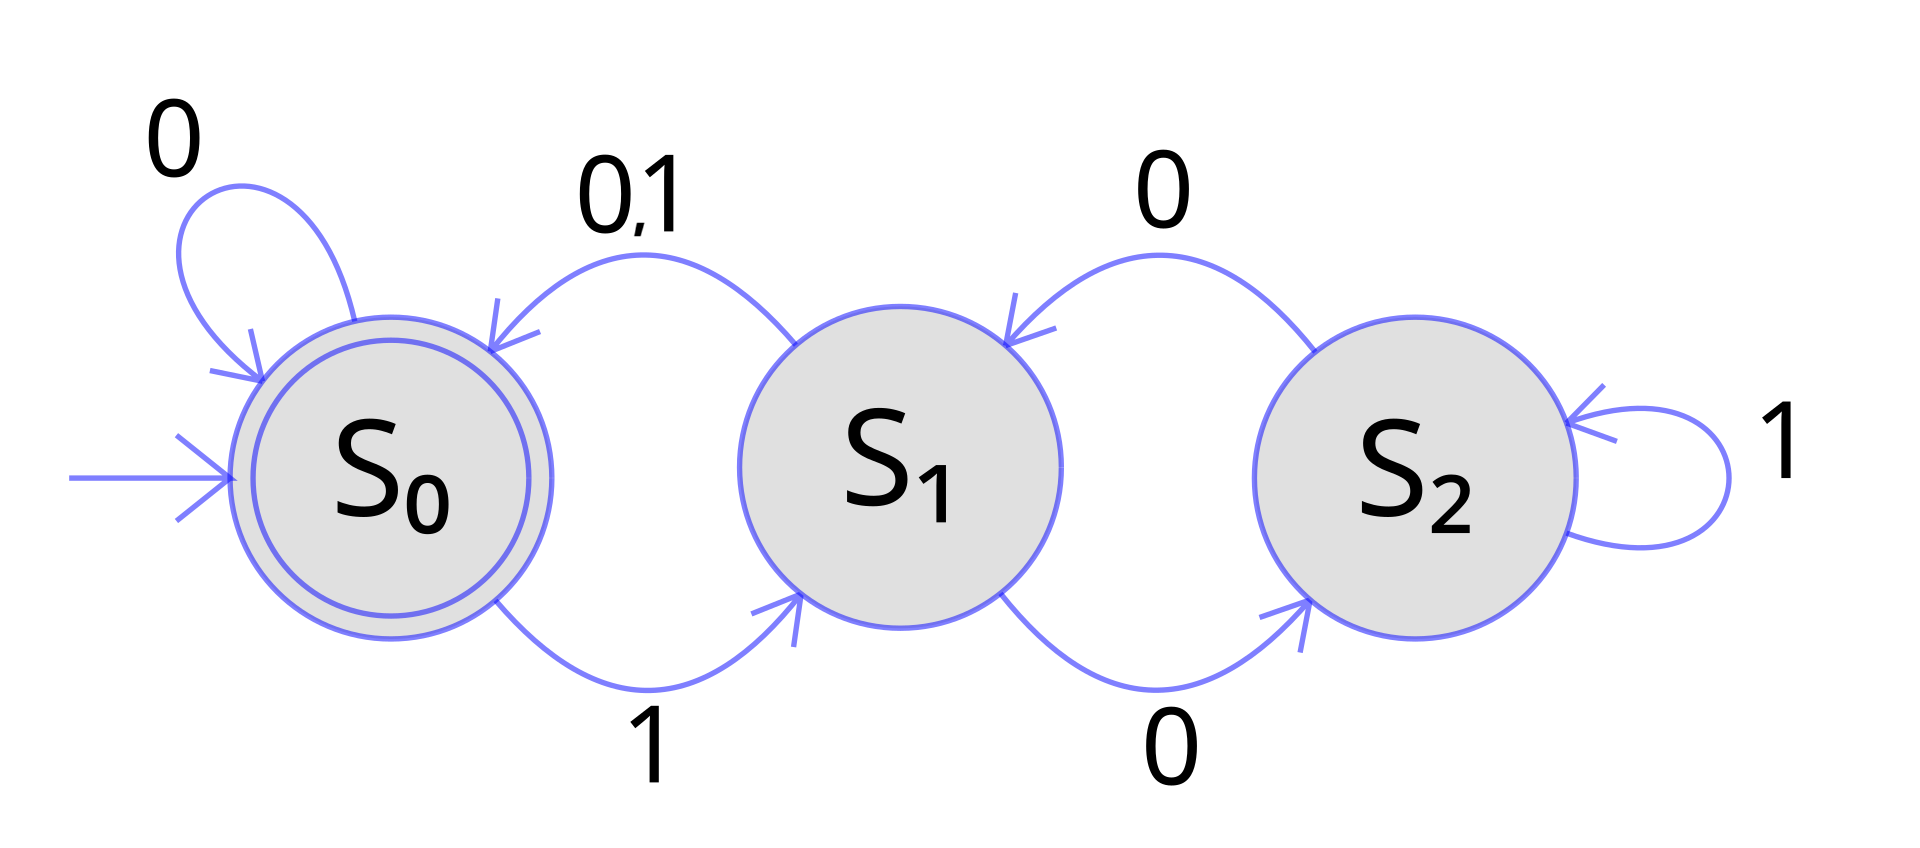
\includegraphics[width=0.6\textwidth]{4. applications/finateStateAutomationsGenNets/images/NDFA.png}
\caption{Пример за недетерминиран краен автомат.}
\label{fig:nfa_figure}
\end{figure}

\paragraph{Кога НКА приема дума?}
\mbox{}\\
Нека $\alpha = a_0 a_1 \cdots a_{n-1} \in \Sigma^*$ е дума. Недетерминираният краен автомат
$\mathcal{N}$ \emph{приема} $\alpha$, ако съществува последователност от състояния
$q_0, q_1, \dots, q_n$, такава че:
\begin{itemize}
	\item $q_0 = q_{\textit{start}}$;
	\item за всяко $i$ с $0 \le i < n$ е изпълнено $q_{i+1} \in \Delta(q_i, a_i)$;
	\item $q_n \in F$.
\end{itemize}
Еквивалентно, чрез разширената преходна функция
\[
	\Delta^* : \mathcal{P}(Q) \times \Sigma^* \;\longrightarrow\;\mathcal{P}(Q),
\]
се казва, че $\alpha$ е приета тогава и само тогава, когато
\[
	\Delta^*(\{q_{\textit{start}}\}, \alpha) \;\cap\; F \;\neq\; \varnothing.
\]

\paragraph{Език на НКА.}
\mbox{}\\
\emph{Езикът, разпознат} от НКА $\mathcal{N}$, е
\[
	L(\mathcal{N}) \;=\; \{\,\alpha \in \Sigma^* \,\mid\, \text{$\mathcal{N}$ приема $\alpha$}\}.
\]

\medskip

\paragraph*{Сравнение между детерминирани и недетерминирани автомати.}
\label{subsec:comparison_dfa_nfa}
\mbox{}\\
Макар ДКА и НКА да се дефинират по различен начин, те разпознават един и същи клас от езици. По-долу се посочват някои основни разлики и добре известният резултат, който ги свързва:
\begin{itemize}
    \item \textbf{Единствена изчислителна пътека (ДКА).}\\
    При \emph{детерминиран} краен автомат за всяко състояние и входен символ съществува точно едно възможно следващо състояние. При обработка на входен низ ДКА следва \emph{единствена} изчислителна пътека от началното към (възможно) приемащо състояние.

    \item \textbf{Паралелна изчислителност (НКА).}\\
    Обратно, \emph{недетерминираният} краен автомат може да има множество възможни следващи състояния за дадена двойка състояние–символ. НКА може да се разглежда като изследващ \emph{всички възможни} изчислителни пътеки паралелно; ако \emph{някоя} от тях достига приемащо състояние, входът се счита приет. Това разклонено поведение често улеснява конструирането на автомати.

    \item \textbf{Интерпретация на ДКА като НКА.}\\
    \emph{Всеки} ДКА може тривиално да се интерпретира като НКА: функцията на прехода връща \emph{множество с точно един елемент}. Следователно ДКА представляват специален случай на НКА с единствен възможен преход на всяка стъпка.

    \item \textbf{Теорема на Рабин–Скот.} \\
    Важна теорема във формалните езици, доказана от Рабин и Скот \cite{rabin-scott}, гласи, че за всеки НКА съществува еквивалентен ДКА, който разпознава същия език. Тази \emph{еквивалентност} обикновено се демонстрира чрез \emph{конструкцията със степенното множество} (\textit{powerset construction}). Идеята е състоянията на новия ДКА да съответстват на \emph{подмножества} от състоянията на оригиналния НКА, като по този начин се улавят всички възможни недетерминирани преходи по детерминиран начин.

    \item \textbf{Защо НКА често се използват като начална стъпка?} \\
    В много теоретични приложения често е \emph{по-лесно} да се проектира НКА благодарение на гъвкавостта му да допуска множество преходи. След като НКА е зададен, при нужда може систематично да се преобразува в ДКА.
\end{itemize}

\subsubsection{Представяне на недетерминирани крайни автомати чрез обобщени мрежи}
\label{sec:simulating_automata_gn}

\hspace*{2.5em}Както беше споменато по-рано, \emph{ОМ} предоставят гъвкава рамка за симулиране на паралелни процеси \cite{Z1,BAM}, което ги прави подходящи за моделиране на начина, по който думите се приемат от автоматите.  
Тук се показва как един \emph{недетерминиран краен автомат} (НКА) може да бъде представен като ОМ.  
Тъй като всеки \emph{детерминиран краен автомат} (ДКА) може лесно да се разглежда като НКА, същата конструкция се прилага и за ДКА с минимални изменения.  
На \textbf{Фигура~\ref{fig:nfa-aa}} е показан индуциран подавтомат, който по-късно се използва като пример.

\begin{figure}[htbp]
	\centering
	\begin{tikzpicture}[>=stealth, scale=1.75]
		% Възли
		\node[circle, draw, minimum size=0.5cm] (A) at (0,0) {$q_1$};
		\node[circle, draw, minimum size=0.5cm] (B) at (2,-1) {$q_2$};
		\node[circle, draw, minimum size=0.5cm] (C) at (2,1) {$q_3$};
		
		% Стрелка към състояние 1 (скрит начален възел)
		\draw[->] (-1,0) -- (A);
		
		% Съществуващи стрелки
		\draw[->] (A) -- node[above] {a} (B);
		\draw[->] (A) -- node[above] {a} (C);
	\end{tikzpicture}
	\captionsetup{width=0.7\textwidth}
	\caption{Индуциран подавтомат с две ребра с етикет \emph{a}, изходящи от едно и също състояние.}
	\label{fig:nfa-aa}
\end{figure}

ОМ се конструира така, че да обхваща всички възможни паралелни изчислителни пътеки на дадения НКА.  
Всеки \emph{преход} в мрежата съответства на едно \emph{състояние} на автомата, а всяка \emph{позиция} в мрежата представлява \emph{ребро} (преходно ребро) на автомата.  
Добавят се и допълнителни преходи и позиции, както е описано по-долу.


\paragraph*{Преходи.}

\begin{itemize}
    \item \textbf{Един преход за всяко състояние на автомата.}\\ За всяко състояние \( q_i \) на НКА се дефинира съответният преход \( Z_i \) в ОМ. Концептуално този преход обработва всички движения от състояние \( q_i \) към неговите следващи състояния, определени от преходната функция на автомата.

    \item \textbf{Краен преход.}\\ Освен преходите, които съпоставят всяко състояние с неговите наследници, се въвежда специален \emph{краен преход} \( Z_{\mathit{final}} \). Този преход позволява на едно \emph{ядро} да \emph{напусне} мрежата, след като автоматът е приел входната дума. Крайният преход има множество входни позиции (свързани с преходите, съответстващи на крайните състояния) и една изходна позиция (която не е входна за никой преход). Ако ядро достигне тази позиция, то това сигнализира за приемане на думата.
\end{itemize}

\paragraph*{Позиции.}

\begin{itemize}
    \item \textbf{Ребра като позиции.}\\ Всяко \emph{ребро} на оригиналния НКА се превръща в \emph{позиция} в мрежата.

    \item \textbf{Входни и изходни позиции.}\\ Ребро от състояние \( q_i \) към \( q_j \) се представя като \emph{изходна} позиция на прехода \( Z_{i} \) и \emph{входна} позиция на прехода \( Z_{j} \).

    \item \textbf{Позиции към крайния преход.}\\ За всяко крайно състояние на НКА се добавя допълнителна изходна позиция от съответния преход, което служи за вход към крайния преход \( Z_{\mathit{final}} \).

    \item \textbf{Начална позиция.}\\ Мрежата съдържа специална начална позиция ($p_{start}$), където първоначално се появява ядро. Тази позиция е входна за прехода, съответстващ на началното състояние на НКА.

    \item \textbf{Крайна позиция.}\\ Мрежата съдържа специална финална позиция, която е единствената изходна позиция на крайния преход \( Z_{\mathit{final}} \). Ядра, достигнали тази позиция, обозначават успешно приемане.
\end{itemize}

\paragraph*{Ядра и техните характеристики.}
\mbox{}\\
В ОМ активните обекти, които се движат между позициите, се наричат \emph{ядра}. В тази конструкция всяко ядро съответства на възможна изчислителна пътека в НКА.

\begin{itemize}
    \item \textbf{Остатък от думата като характеристика.}\\ Всяко ядро носи като своя \emph{характеристика} непрочетената част от входната дума, означена като „\texttt{word}“. Първоначално тази характеристика е цялата входна дума \( w = a_0 a_1 \cdots a_{n-1} \).

    \item \textbf{Характеристични функции на позициите.}\\ Всяка изходна позиция на преход в мрежата има характеристична функция, която актуализира непрочетената дума: при преминаване през позиция, различна от началната, първият символ на думата се премахва. За позицията, през която ядро влиза от $p_{start}$, символ не се премахва.

    \item \textbf{Паралелни пътеки.}\\  Ако НКА се разклонява към няколко наследника, ядрото се дублира в няколко копия с еднакъв текущ остатък на думата.

    \item \textbf{Празен низ.}\\ Когато характеристиката „\texttt{word}“ стане празна, целият вход е обработен. Ако ядрото е на изходна позиция, свързана с крайно състояние, то може да премине към крайния преход \( Z_{\mathit{final}} \) и да напусне мрежата, отбелязвайки приемане.
\end{itemize}

\paragraph*{Илюстрация на движението на ядрата.}
\mbox{}\\
Разглежда се примерът от \textbf{Фигура~\ref{fig:nfa-aa}}, където едно състояние на НКА има две ребра с етикет „a“, водещи към различни състояния (например \(q_2\) и \(q_3\)).  
В ОМ ядрото се \emph{разделя} на две ядра, всяко от които носи един и същ остатък от входната дума.  
Нека първоначалната дума е \(a\alpha\) с \(\alpha \in \Sigma^*\). След разделянето двете ядра запазват същия остатък \(a\alpha\).

На \textbf{Фигура~\ref{fig:gn-nfa}} е показана ОМ, съответстваща на индуцирания НКА, в състояние с две активни ядра преди изпълнението на стъпка.
\newpage
\begin{figure}[ht]
  \centering
  \tiny
  \setlength{\unitlength}{16pt}
  \begin{picture}(15.06,9.07)
    \linethickness{0.4pt}
    % --- Transitions ---
    \put(3.18,9.37){\makebox(0,0)[b]{$Z_1$}}
    \put(3.18,8.00){\makebox(0,0)[bb]{\Large$\bigtriangledown$}}
    \put(3.18,8.00){\line(0,-1){8.00}}
    \put(11.89,9.37){\makebox(0,0)[b]{$Z_2$}}
    \put(11.91,8.00){\makebox(0,0)[bb]{\Large$\bigtriangledown$}}
    \put(11.91,8.00){\line(0,-1){3.00}}
    \put(11.89,4.37){\makebox(0,0)[b]{$Z_3$}}
    \put(11.91,3.00){\makebox(0,0)[bb]{\Large$\bigtriangledown$}}
    \put(11.91,3.00){\line(0,-1){3.00}}
    % --- Places ---
    \put(6.33,7.13){\makebox(0,0)[cc]{$p_{1-2}$}}
    \put(6.33,6.33){\circle{1.0}}
    \put(6.33,6.33){\circle*{0.4}}

    \put(6.32,2.46){\makebox(0,0)[cc]{$p_{1-3}$}}
    \put(6.32,1.67){\circle{1.0}}
    \put(6.32,1.67){\circle*{0.4}}
    \put(15.06,7.13){\makebox(0,0)[cc]{$p_{2-y}$}}
    \put(15.06,6.33){\circle{1.0}}
    \put(15.06,2.46){\makebox(0,0)[cc]{$p_{3-z}$}}
    \put(15.06,1.67){\circle{1.0}}
    \put(0.00,4.79){\makebox(0,0)[cc]{$p_{x-1}$}}
    \put(0.00,4.00){\circle{1.0}}
    % --- Edges ---
    % Z1 -> p2
    \put(3.20,6.33){\vector(1,0){2.63}}
    % Z1 -> p3
    \put(3.20,1.67){\vector(1,0){2.62}}
    % Z2 -> p4
    \put(11.94,6.33){\vector(1,0){2.62}}
    % Z3 -> p5
    \put(11.94,1.67){\vector(1,0){2.62}}
    % p1 -> Z1
    \put(0.50,4.00){\vector(1,0){2.65}}
    % p2 -> Z2
    \put(6.83,6.33){\vector(1,0){5.06}}
    % p3 -> Z3
    \put(6.82,1.67){\vector(1,0){5.07}}
  \end{picture}
  \normalsize
  \captionsetup{width=0.8\textwidth}
  \caption{ОМ, съответстваща на индуцирания НКА от \textbf{Фигура~~\ref{fig:nfa-aa}}, с две активни ядра ПРЕДИ стъпка.}
  \label{fig:gn-nfa}
\end{figure}

За имената на позициите се използва конвенцията \( p_{\text{origin-destination}} \).  
При следващото преместване ядрата се придвижват към $p_{2-y}$ и $p_{3-z}$.  
Характеристичните функции на тези позиции премахват първия символ от думата; следователно, и двете ядра ще носят актуализирания остатък \(\alpha\), както е показано на \textbf{Фигура~\ref{fig:gn-nfa-after-step}}.

\begin{figure}[ht]
  \centering
  \tiny
  \setlength{\unitlength}{16pt}
  \begin{picture}(15.06,9.07)
    \linethickness{0.4pt}
    % --- Transitions ---
    \put(3.18,9.37){\makebox(0,0)[b]{$Z_1$}}
    \put(3.18,8.00){\makebox(0,0)[bb]{\Large$\bigtriangledown$}}
    \put(3.18,8.00){\line(0,-1){8.00}}
    \put(11.89,9.37){\makebox(0,0)[b]{$Z_2$}}
    \put(11.91,8.00){\makebox(0,0)[bb]{\Large$\bigtriangledown$}}
    \put(11.91,8.00){\line(0,-1){3.00}}
    \put(11.89,4.37){\makebox(0,0)[b]{$Z_3$}}
    \put(11.91,3.00){\makebox(0,0)[bb]{\Large$\bigtriangledown$}}
    \put(11.91,3.00){\line(0,-1){3.00}}
    % --- Places ---
    \put(6.33,7.13){\makebox(0,0)[cc]{$p_{1-2}$}}
    \put(6.33,6.33){\circle{1.0}}

    \put(6.32,2.46){\makebox(0,0)[cc]{$p_{1-3}$}}
    \put(6.32,1.67){\circle{1.0}}

    \put(15.06,7.13){\makebox(0,0)[cc]{$p_{2-y}$}}
    \put(15.06,6.33){\circle{1.0}}
    \put(15.06,6.33){\circle*{0.4}}
    \put(15.06,2.46){\makebox(0,0)[cc]{$p_{3-z}$}}
    \put(15.06,1.67){\circle{1.0}}
    \put(15.06,1.67){\circle*{0.4}}
    \put(0.00,4.79){\makebox(0,0)[cc]{$p_{x-1}$}}
    \put(0.00,4.00){\circle{1.0}}
    % --- Edges ---
    % Z1 -> p2
    \put(3.20,6.33){\vector(1,0){2.63}}
    % Z1 -> p3
    \put(3.20,1.67){\vector(1,0){2.62}}
    % Z2 -> p4
    \put(11.94,6.33){\vector(1,0){2.62}}
    % Z3 -> p5
    \put(11.94,1.67){\vector(1,0){2.62}}
    % p1 -> Z1
    \put(0.50,4.00){\vector(1,0){2.65}}
    % p2 -> Z2
    \put(6.83,6.33){\vector(1,0){5.06}}
    % p3 -> Z3
    \put(6.82,1.67){\vector(1,0){5.07}}
  \end{picture}
  \normalsize
  \captionsetup{width=0.8\textwidth}
  \caption{ОМ, съответстваща на индуцирания НКА от \textbf{Фигура~~\ref{fig:nfa-aa}}, с две активни ядра СЛЕД стъпка.}
  \label{fig:gn-nfa-after-step}
\end{figure}

\paragraph*{Индексирани матрици.}
\mbox{}\\
По-долу се описва как се конструират \emph{индексираните матрици} на ОМ, която симулира зададен НКА \((Q, \Sigma, \delta, q_{start}, F)\).

\paragraph*{Дефиниция на основен предикат.}
\mbox{}\\
Въвежда се следният предикат, използван в индексираните матрици:
\[
S(x,y)\;\Longleftrightarrow\;
\begin{aligned}
&\text{характеристиката „\textit{Word}“ на ядрото е от вида } aw, 
a \in \Sigma,\; w \in \Sigma^{*} \\[0.4mm]
&\text{и } q_{y} \in \delta(q_{x}, a).
\end{aligned}
\]

Тук $q_x$ съответства на състоянието на НКА, свързано с входната позиция $p_x$ в прехода на ОМ, а $q_y$ е състоянието, свързано с изходната позиция $p_y$. Следователно, предикатът $S(x,y)$ е истина точно когато ядрото на позиция $p_x$ може при вход $a$ да премине в състояние $q_y$ в НКА, като характеристичната дума се обновява от $aw$ до $w$.


\paragraph{Преход $Z_i$ за нефинално състояние $q_i$.}
\mbox{}\\
За всяко състояние $q_i \in Q$ нека \textit{Input}$(q_i)$ е множеството от състояния на НКА, които имат директен преход (ребро) към $q_i$, а \textit{Output}$(q_i)$ – множеството от състояния, към които съществува преход (ребро) от $q_i$.  
В ОМ тези ще съответстват съответно на входните и изходните позиции на прехода $Z_i$.  
Формално, индексираната матрица на $Z_i$ има редове, съответстващи на позициите в \textit{Input}$(q_i)$, и колони, съответстващи на позициите в \textit{Output}$(q_i)$.

Следователно индексираната матрица за прехода $Z_i$ е:

\[
\begin{array}{c|c}
    & p_{i-y} \quad \text{където } q_y \in \textit{Output}(q_i) \\ \hline
p_{x-i} \quad \text{където } q_x \in \textit{Input}(q_i) & S(x,i)
\end{array}
\]


\paragraph{Преход на началното състояние с допълнителна позиция.}
\mbox{}\\
За прехода, който съответства на началното състояние, се въвежда допълнителна позиция $p_{\text{start}}$, от която започва симулацията.  
Всяко ядро в $p_{\text{start}}$ може безусловно да се премести в някоя от позициите, които съответстват на \textit{Output}$(q_{\text{start}})$.  
Следователно в индексираната матрица за прехода на началното състояние има допълнителен ред за $p_{\text{start}}$, в който всички елементи са зададени като $\text{\textit{True}}$:

\[
\resizebox{0.4\textwidth}{!}{$
\begin{array}{c|cccc}
    & \dots &   &   & \dots \\ \hline
\vdots & \ddots & & & \vdots \\[6pt]
p_{\text{start}} & \text{True} & \text{True} & \cdots & \text{True} \\
\end{array}
$}
\]

\paragraph{Допълнителна изходна позиция за крайните състояния.}
\mbox{}\\
За всеки преход $Z_i$, който съответства на крайно състояние $q_i \in F$, се въвежда допълнителна изходна позиция $p_{i,\text{final}}$, която служи като вход към крайния „приемащ“ преход $Z_{\text{final}}$.  
Преминаването от прехода \(Z_i\) към \(p_{i,\text{final}}\) е винаги разрешено (т.е. предикатът е $\text{\textit{True}}$).  
В резултат за всеки такъв $Z_i$ индексираната матрица има допълнителна колона, съответстваща на $p_{i,\text{final}}$, в която всеки елемент (в тази колона) е зададен като $\text{\textit{True}}$:

\begin{center}
\resizebox{0.3\textwidth}{!}{
$\begin{array}{c|ccc}
      & \dots & \dots & p_{i,\text{final}} \\ \hline
\vdots & \ddots & \ddots & \text{True} \\
\vdots & \ddots & \ddots & \vdots      \\
\vdots & \ddots & \ddots & \text{True} \\
\end{array}$
}
\end{center}

\paragraph{Краен преход ($Z_{\text{final}}$).}
\mbox{}\\
Накрая се дефинира глобалният краен преход $Z_{\text{final}}$.  
Този преход взема ядра от позициите $p_{t,\text{final}}$, където $q_t \in F$, и ги премества в една „приемаща“ изходна позиция $P_{\text{final}}$.  
За да бъде входната дума приета от симулацията на НКА, характеристичната дума на ядрото трябва да бъде празна. 
За тази цел се използва предикатът:

\[
E \;\;\Longleftrightarrow\;\; \text{характеристичната „дума“ на ядрото е празна.}
\]

Следователно индексираната матрица за $Z_{\text{final}}$ е:

\begin{center}
\resizebox{0.35\textwidth}{!}{
  $\begin{array}{c|c}
       & P_{\text{final}} \\ \hline
   p_{t,\text{final}} \ (q_t \in F) & E
   \end{array}$
}
\end{center}

Ако предикатът $E$ е изпълнен, ядрото се премества в $P_{\text{final}}$, което показва, че симулираният НКА е приел първоначалната входна дума.

\paragraph*{Поток в обобщената мрежа.}
\begin{enumerate}
    \item \textbf{Инициализация.}\\ Едно ядро влиза в ОМ с характеристика, зададена като цялата входна дума \(\alpha\). Това ядро се поставя във входната позиция на ОМ, която съответства на \emph{началното състояние} на НКА.
    
    \item \textbf{Преходи между състояния.}\\ При всеки преход на ОМ \( Z_q \), логиката на предикатите проверява дали следващият входен символ на ядрото съответства на допустим преход от \( q \) към друго състояние \( q' \). Ако е така, ядрото се премества в съответната \emph{позиция} (която представя реброто \( q \rightarrow q' \)). Характеристичната дума на ядрото се обновява чрез премахване на консумирания символ.
    
    \item \textbf{Разклоняване.}\\ Ако съществуват множество допустими преходи от \( q \) (отразяващи недетерминираността на НКА), от \( Z_q \) могат да излязат няколко ядра  всяко със същата характеристична дума, но водещо към различни последващи преходи в ОМ.
    
    \item \textbf{Приемане.}\\ Ако ядрото има празна характеристична дума и се намира (или може да се премести) в позиция, съответстваща на крайно състояние на НКА, то се насочва към \emph{крайния преход} \( Z_{\mathit{final}} \). Оттам то \emph{излиза} от ОМ, което означава успешно приемане на входната дума.
\end{enumerate}
\hspace*{2.5em}При следването на тези стъпки ОМ ефективно симулира всички възможни изчислителни пътища на НКА паралелно. Следователно думата се приема точно тогава, когато поне едно ядро достигне и премине през крайния преход. Този модел подчертава гъвкавостта на ОМ при симулация не само на чисто \emph{детерминирани} механизми (ДКА), но и на системи, изискващи \emph{паралелно изследване} на състоянията (НКА).

\bigskip
\noindent

\begin{Theorem}\label{thm:nka-om}
Всеки недетерминиран краен автомат (НКА) може да бъде представен чрез съответна обобщена мрежа (ОМ).
\end{Theorem}

\renewcommand{\proofname}{Доказателство}
\begin{proof}
Нека $A$ е произволен НКА, $q_i$ е произволно негово състояние и $q_j$ е такова състояние, че $q_i \in \Delta(q_j,a)$ за някое $a \in \Sigma$.

В гореописаната конструкция разглеждаме прехода в ОМ, който съответства на $q_i$. Предикатът на прехода е изпълнен точно тогава когато характеристиката \texttt{word} започва със символ $a$. Характеристичните функции на позициите, излизащи от прехода, премахват първия символ на \texttt{word}, т.е. преобразуват $aw$ във $w$. Следователно активирането на този преход реализира същата обработка на входната дума, както преходът $q_j \xrightarrow{a} q_i$ в автомата, и съответства точно на поведението на състоянията в НКА.

По \textbf{Теоремата за пълнота на преходите в ОМ} всяка ОМ се получава като обединение на своите преходи; следователно мрежата, получена чрез посочената процедура, е коректно изградена като обединение на съответните преходи и представлява завършен модел \cite{Z1, BAM}.

Следователно всеки НКА може да бъде представен чрез съответна ОМ, което доказва твърдението.
\end{proof}


\subsubsection{Подробен пример за недетерминиран краен автомат, представен като обобщена мрежа}

\hspace*{2.5em}По-долу е показан подробен пример за ОМ, съответстваща на недетерминиран краен автомат (НКА) с две крайни състояния $q_3$ и $q_5$ (\textbf{Фигура~\ref{fig:nka-two-finals}}).

\begin{figure}[H]
\centering
\begin{tikzpicture}[>=Latex, scale=1.75]

    % State q_1
    \node[draw, circle, minimum size=0.5cm, inner sep=0pt] (n1) at (0,4) {};
    \node[below=0.1cm of n1] {$q_1$};

    % State q_2
    \node[draw, circle, minimum size=0.5cm, inner sep=0pt] (n2) at (2,4) {};
    \node[below=0.1cm of n2] {$q_2$};

    % State q_3 (final)
    \node[draw, circle, double, minimum size=0.5cm, inner sep=0pt] (n3) at (4,4) {};
    \node[below=0.1cm of n3] {$q_3$};

    % State q_4
    \node[draw, circle, minimum size=0.5cm, inner sep=0pt] (n4) at (4,6) {};
    \node[below=0.1cm of n4] {$q_4$};

    % State q_5 (final)
    \node[draw, circle, double, minimum size=0.5cm, inner sep=0pt] (n5) at (6,6) {};
    \node[below=0.1cm of n5] {$q_5$};

    % Arrow from nowhere to q_1
    \draw[->] (-1,4) -- (n1);

    % Transitions
    \draw[->, bend left=15] (n1) to node[above] {a} (n2);
    \draw[->] (n2) -- node[below] {b} (n3);
    \draw[->] (n2) -- node[left] {b} (n4);
    \draw[->, bend left=20] (n4) to node[above] {a} (n5);
    \draw[->] (n4) to[out=120,in=60,loop] node[above] {b} (n4);
    \draw[->, bend right=30] (n3) to node[above] {b} (n2);

\end{tikzpicture}
\caption{Примерен НКА с две крайни състояния: $q_3$ и $q_5$.}
\label{fig:nka-two-finals}
\end{figure}
Езикът на този автомат може да бъде представен чрез регулярния израз:
\[
a \,(bb)^* \Bigl(b + b^+\,a\Bigr).
\]

Автоматът е недетерминиран, защото от състояние $q_2$ излизат две ребра с етикет „b“. На \textbf{Фигура~\ref{fig:om-sim}} е представена ОМ, симулираща този автомат.
\newpage

\begin{figure}[htbp]
\centering
\setlength{\unitlength}{12pt}%
{\tiny
	\begin{picture}(30.29,17.27)
	\linethickness{0.4pt}

% --- Transitions (unchanged) ---
\put(3.85,17.77){\makebox(0,0)[b]{$Z_1$}}
\put(3.87,16.38){\makebox(0,0)[bb]{\Large$\bigtriangledown$}}
\put(3.87,16.38){\line(0,-1){3.32}}

\put(9.91,17.77){\makebox(0,0)[b]{$Z_2$}}
\put(9.92,16.38){\makebox(0,0)[bb]{\Large$\bigtriangledown$}}
\put(9.92,16.38){\line(0,-1){6.65}}

\put(15.98,17.77){\makebox(0,0)[b]{$Z_4$}}
\put(15.99,16.38){\makebox(0,0)[bb]{\Large$\bigtriangledown$}}
\put(15.99,16.38){\line(0,-1){6.65}}

\put(22.05,17.77){\makebox(0,0)[b]{$Z_5$}}
\put(22.06,16.38){\makebox(0,0)[bb]{\Large$\bigtriangledown$}}
\put(22.06,16.38){\line(0,-1){3.32}}

\put(28.11,17.77){\makebox(0,0)[b]{$Z_{\text{final}}$}}
\put(28.12,16.38){\makebox(0,0)[bb]{\Large$\bigtriangledown$}}
\put(28.12,16.38){\line(0,-1){6.65}}

\put(15.98,8.55){\makebox(0,0)[b]{$Z_3$}}
\put(15.99,7.15){\makebox(0,0)[bb]{\Large$\bigtriangledown$}}
\put(15.99,7.15){\line(0,-1){6.65}}

% --- Places (unchanged) ---
\put(6.05,15.25){\makebox(0,0)[cc]{$p_{1-2}$}} \put(6.05,14.53){\circle{1}}

\put(12.11,12.47){\makebox(0,0)[cc]{$p_{2-3}$}} \put(12.11,11.77){\circle{1}}

\put(12.11,15.25){\makebox(0,0)[cc]{$p_{2-4}$}} \put(12.11,14.53){\circle{1}}

\put(18.18,15.25){\makebox(0,0)[cc]{$p_{4-5}$}} \put(18.18,14.53){\circle{1}}

\put(18.18,12.47){\makebox(0,0)[cc]{$p_{4-4}$}} \put(18.18,11.77){\circle{1}}

\put(24.25,15.25){\makebox(0,0)[cc]{$p_{5-fin}$}} \put(24.25,14.53){\circle{1}}

\put(30.29,15.25){\makebox(0,0)[cc]{$p_{fin}$}} \put(30.29,14.53){\circle{1}}

\put(18.18,6.01){\makebox(0,0)[cc]{$p_{3-fin}$}} \put(18.18,5.31){\circle{1}}

\put(18.18,3.25){\makebox(0,0)[cc]{$p_{3-2}$}} \put(18.18,2.54){\circle{1}}

\put(0.00,15.25){\makebox(0,0)[cc]{$p_{start}$}}
\put(0.00,14.53){\circle{1}}


% --- From transitions to places ---
%% Z1 -> p1-2
\put(3.87,14.53){\vector(1,0){1.68}}
%% Z2 -> p2-3
\put(9.94,11.77){\vector(1,0){1.67}} % shortened from 1.83
%% Z2 -> p3-3
\put(9.94,14.53){\vector(1,0){1.67}} % shortened from 1.83
%% Z4 -> p4-5
\put(16.01,14.53){\vector(1,0){1.67}} % shortened from 1.83
%% Z4 -> p4-4
\put(16.01,11.77){\vector(1,0){1.67}} % shortened from 1.83
%% Z5 -> p5-fin
\put(22.08,14.53){\vector(1,0){1.67}} % shortened from 1.83
%% Z_final -> p-fin
\put(28.14,14.53){\vector(1,0){1.65}} % shortened from 1.83
%% Z3 -> p3-fin
\put(16.01,5.31){\vector(1,0){1.67}}  % shortened from 1.83
%% Z3 -> p3-2
\put(16.01,2.54){\vector(1,0){1.67}}  % shortened from 1.83

% --- From places to transitions ---
%% p_start -> Z1
\put(0.50,14.53){\line(1,0){1.65}}    % start shifted from 0.33
\put(2.15,14.53){\vector(1,0){1.71}}

%% p1-2 -> Z2
\put(6.55,14.53){\line(1,0){1.65}}    % start shifted from 6.38
\put(8.20,14.53){\vector(1,0){1.71}}

%% p3-2 -> Z2
\put(18.18,2.04){\line(0,-1){2.04}}   % shortened from 2.21
\put(18.18,0.00){\line(-1,0){9.95}}
\put(8.23,0.00){\line(0,1){11.77}}
\put(8.23,11.77){\vector(1,0){1.69}}

%% p2-3 -> Z3
\put(12.11,11.27){\line(0,-1){5.96}}  % start shifted from 11.44
\put(12.11,5.31){\line(1,0){3.79}}
\put(15.90,5.31){\vector(1,0){0.13}}

%% p3-3 -> Z4
\put(12.61,14.53){\vector(1,0){3.37}} % start shifted from 12.44

%% p4-4 -> Z4
\put(18.18,11.27){\line(0,-1){2.04}}  % shortened from 2.21
\put(18.18,9.23){\line(-1,0){3.88}}
\put(14.30,9.23){\line(0,1){2.54}}
\put(14.30,11.77){\vector(1,0){1.69}}

%% p4-5 -> Z5
\put(18.68,14.53){\line(1,0){1.63}}   % start shifted from 18.51
\put(20.31,14.53){\vector(1,0){1.74}}

%% p3-fin -> Z_final
\put(18.68,5.31){\line(1,0){3.38}}    % start shifted from 18.51
\put(22.06,5.31){\line(0,1){6.46}}
\put(22.06,11.77){\vector(1,0){6.05}}

%% p5-fin -> Z_final
\put(24.75,14.53){\vector(1,0){3.35}} % start shifted from 24.58

\end{picture}
}

\caption{Обобщена мрежа, която симулира дадения автомат.}
\label{fig:om-sim}
\end{figure}

Както беше описано, има по един преход за всяко състояние ($Z_1, Z_2, Z_3, Z_4, Z_5$) и един допълнителен краен преход ($Z_{\text{final}}$).

\subsubsection{Симулация на множество недетерминирани крайни автомати чрез една обобщена мрежа}

\hspace*{2.5em}В този подраздел се показва, че краен набор от недетерминирани крайни автомати (НКА) може да бъде представена чрез една ОМ.  
Тази форма на представяне позволява едновременно проверяване на входни низове през множество НКА чрез една единствена ОМ.

\begin{Observation}
Всяко крайно множество от НКА може да бъде представено чрез една обобщена мрежа.
\end{Observation}

\renewcommand{\proofname}{Доказателство}
\begin{proof}
Беше показано, че всеки отделен НКА може да бъде симулиран чрез съответна ОМ.  
Освен това, според една теорема, ако $E_1$ и $E_2$ са ОМ, то тяхното обединение $E_1 \cup E_2$ също е ОМ~\cite{Z1}.  
Следователно, чрез обединяване на ОМ, съответстващи на всеки НКА от крайното множество, се получава една ОМ, която представя съвкупно всички разглеждани НКА.
\end{proof}

\subsubsection{Симулация на един недетерминиран краен автомат с помощта на \textit{OnlineGN}}
\label{subsec:simulation_steps}

\hspace*{2.5em}В този пример беше представен НКА и беше построена съответната ОМ, която разпознава език, съдържащ думата \texttt{abbba}.  
По-долу се демонстрира как да стартираме тази ОМ в инструмента \textit{OnlineGN}.  
В симулацията се използва леко изменена нотация (тъй като долни индекси не се поддържат).  
Например, $q_{i-j}$ се изписва като \texttt{qi-j}.

\begin{figure}[H]
	\centering
	\setlength{\fboxrule}{2pt}
	\setlength{\fboxsep}{0pt}
	\fbox{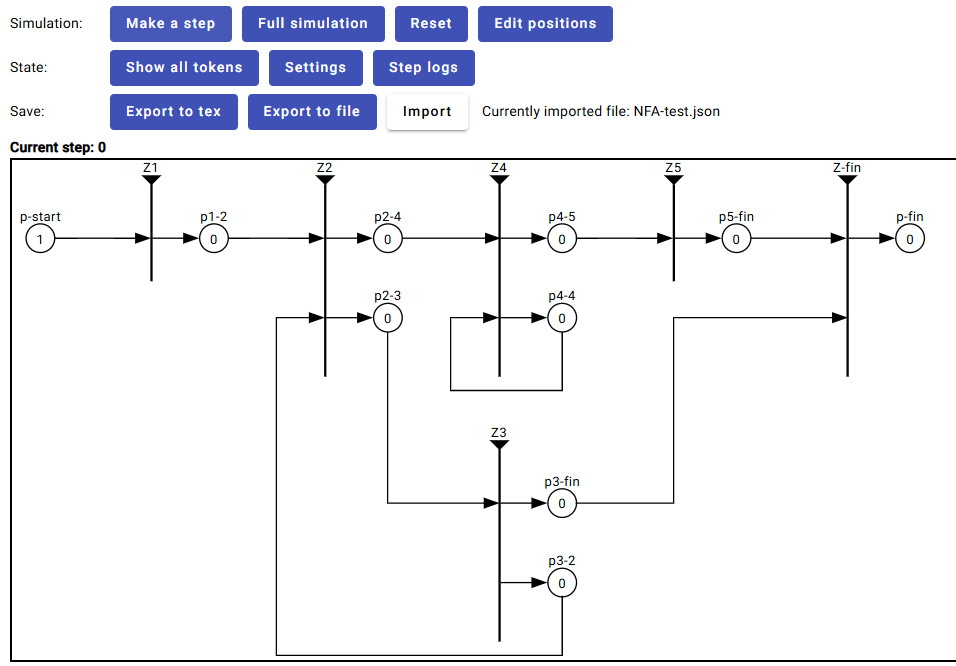
\includegraphics[width=1\textwidth]{4. applications/finateStateAutomationsGenNets/images/NFA-OGN-1.PNG}}
	\caption{Начална конфигурация на ОМ с едно ядро в началната позиция (\texttt{p-start}).}
	\label{fig:gn_initial_setup}
\end{figure}

\vspace{0.2cm}

Както е показано на \textbf{Фигура~\ref{fig:gn_initial_setup}}, ОМ започва с едно ядро в началната позиция \texttt{p-start}.
Началното ядро, носещо пълната входна дума \texttt{abbba}, е показано на \textbf{Фигура~\ref{fig:gn_token_start}}.


\begin{figure}[H]
	\centering
	\setlength{\fboxrule}{2pt}
	\setlength{\fboxsep}{0pt}
	\fbox{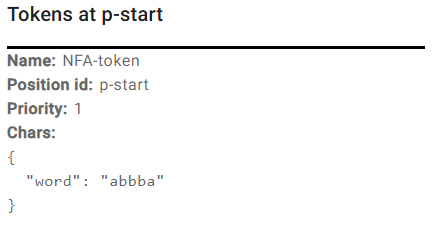
\includegraphics[width=0.6\textwidth]{4. applications/finateStateAutomationsGenNets/images/NFA-OGN-2.PNG}}
	\caption{Ядро в \texttt{p-start} с характеристика \texttt{abbba}.}
	\label{fig:gn_token_start}
\end{figure}

При първата стъпка от симулацията ядрото преминава от \texttt{p-start} към позиция \texttt{p1-2} (вж. \textbf{Фигури~\ref{fig:gn_first_transition}} и~\textbf{\ref{fig:gn_first_transition_zoom}}).  
Отбелязва се, че характеристиката на ядрото остава непроменена след това начално преместване, тъй като обработката на входните символи (т.е. премахването на символи) все още не е започнала.


\begin{figure}[H]
	\centering
	\setlength{\fboxrule}{2pt}
	\setlength{\fboxsep}{0pt}
	\fbox{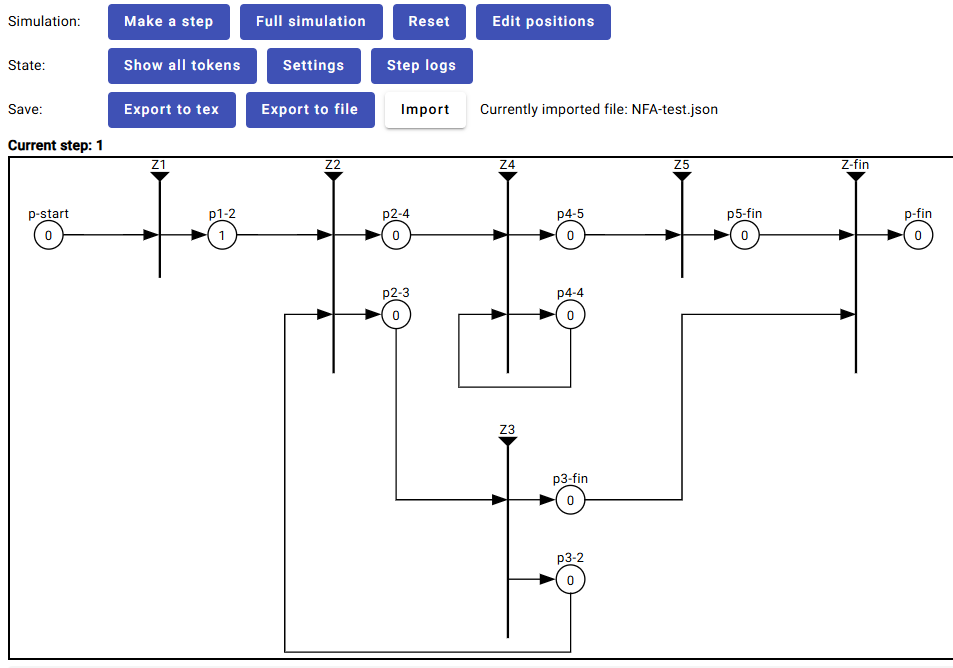
\includegraphics[width=1\textwidth]{4. applications/finateStateAutomationsGenNets/images/NFA-OGN-3.PNG}}
	\caption{След първата стъпка ядрото е в \texttt{p1-2}.}
	\label{fig:gn_first_transition}
\end{figure}


\begin{figure}[H]
	\centering
	\setlength{\fboxrule}{2pt}
	\setlength{\fboxsep}{0pt}
	\fbox{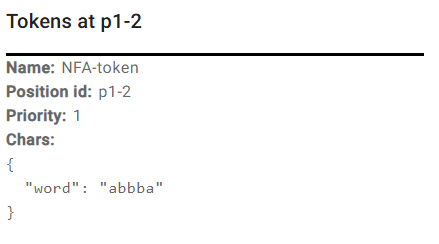
\includegraphics[width=0.6\textwidth]{4. applications/finateStateAutomationsGenNets/images/NFA-OGN-4.PNG}}
	\captionsetup{width=0.8\textwidth}
	\caption{Увеличен изглед на ядрото в \texttt{p1-2}, все още с характеристика \texttt{abbba}.}
	\label{fig:gn_first_transition_zoom}
\end{figure}

Следващите стъпки в ОМ съответстват на последователно прочитане на всеки символ от думата \texttt{abbba} и преминаване през съответните преходи.  
Накрая, след като всички символи бъдат прочетени, ядрото се насочва към крайната позиция \texttt{p-fin}, както е показано на \textbf{Фигура~\ref{fig:gn_final_state}}.

\begin{figure}[H]
	\centering
	\setlength{\fboxrule}{2pt}
	\setlength{\fboxsep}{0pt}
	\fbox{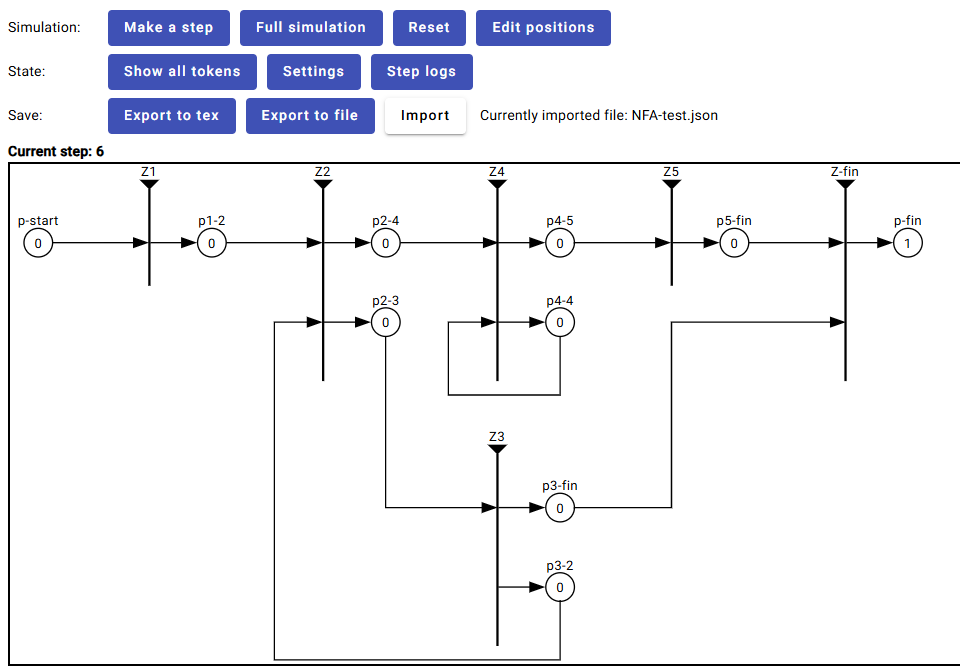
\includegraphics[width=1\textwidth]{4. applications/finateStateAutomationsGenNets/images/NFA-OGN-5.PNG}}
	\caption{Ядрото е достигнало крайната позиция \texttt{p-fin}.}
	\label{fig:gn_final_state}
\end{figure}

Когато ядрото достигне крайната позиция \texttt{p-fin}, неговата характеристика става празен низ, което показва, че цялата дума \texttt{abbba} е разпозната (или „приета“) от ОМ/\linebreak НКА, както е показано на \textbf{Фигура~\ref{fig:gn_empty_characteristic}}.

\begin{figure}[H]
	\centering
	\setlength{\fboxrule}{2pt}
	\setlength{\fboxsep}{0pt}
	\fbox{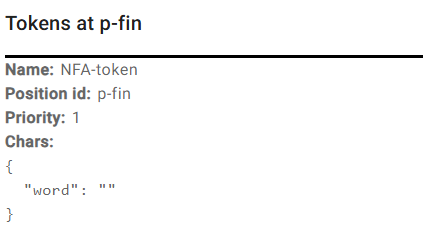
\includegraphics[width=0.6\textwidth]{4. applications/finateStateAutomationsGenNets/images/NFA-OGN-6.PNG}}
	\captionsetup{width=0.7\textwidth}
	\caption{Характеристиката на ядрото става празен низ при приемане.}
	\label{fig:gn_empty_characteristic}
\end{figure}

Тази поредица от стъпки демонстрира как инструментът \textbf{\textit{OnlineGN}} може да се използва за визуализиране и проследяване на движението на ядрата и развитието на техните характеристики (входните символи) през ОМ, моделираща НКА.

\subsubsection{Заключение}

\hspace*{2.5em}В тази глава беше представено как ОМ могат да бъдат използвани за симулация както на детерминирани, така и на недетерминирани крайни автомати.  
Чрез свързване на всяко състояние от автомата с преход в ОМ и представяне на ребрата като позиции, ефективно се улавят всички паралелни изчислителни пътища, които един НКА може да следва.

Архитектурата, базирана на ядра, позволява лесно моделиране на разклонения и едновременна обработка на множество състояния.  
Този подход демонстрира гъвкавостта и устойчивостта на ОМ в теорията на формалните езици и изчисленията, базирани на автомати, като открива възможности за бъдещи приложения в области, където паралелната обработка и конкурентността имат съществена роля.